\documentclass[12pt,a4paper]{article}
\usepackage{fullpage}
\pagestyle{plain}
% choose any of the following packages to support AmsTeX
%\usepackage{amsmath,amssymb,amsfonts,mathrsfs,mathptm,bm,mathtools}
% choose the following package to insert eps figures
% for png, jpg or pdf figures, use pdflatex
\usepackage{graphicx}
\graphicspath{{./img}}

\newcommand{\question}[1]{\bigskip\noindent{\textbf{Q{#1} solution}}}

% set HW number
\newcommand{\HWnum}{3}
% specify first and last name and the ID number of students in the group
% append asterix to indicate who is making the submission
\newcommand{\StudentA}{Hanggang Zhu$^\ast$, 3200110457}
\newcommand{\StudentB}{Suhao Wang, 3200110777}
\newcommand{\StudentC}{Lumeng Xu 3200110184}

% ===============================================================
\begin{document}

%%% header
{\noindent \rule{\linewidth}{0.2mm}}
\noindent{ECE 374, ZJUI, Spring 2023\hfill%
  \textbf{\large H{}W\HWnum\ Solutions} \hfill \today\smallskip}

\noindent{\hfill \StudentA, \StudentB, and \StudentC \hfill}
\\[-0.2cm]{\noindent \rule{\linewidth}{0.2mm}}
%%% end header


\question{7.A}

The follwing NFA accpets the language. On reading 3,7,4 at states $q_0,q_1,q_2$ respectively, The NFA can go to next state. In all states the NFA can stay at current state reading any character. But accepting state is reached only if $3,7,4$ are read as a subsequence.


\begin{figure}[hbt!]
	\centering
	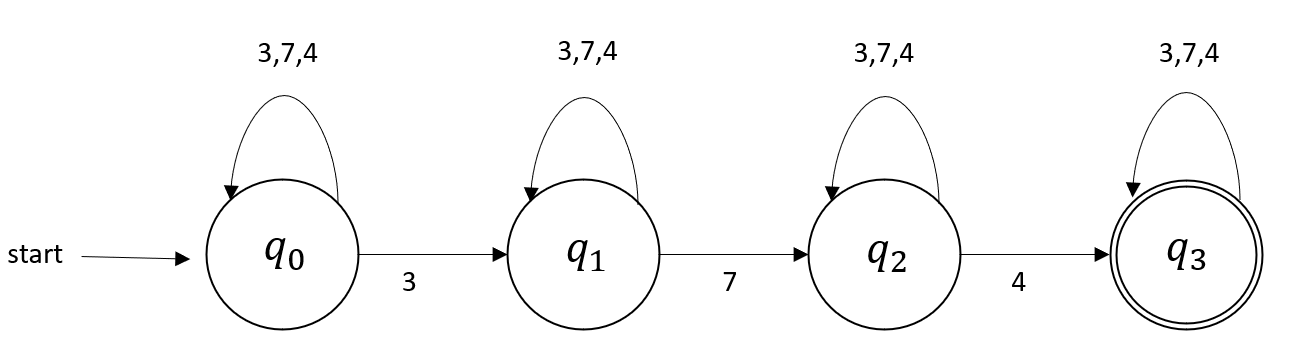
\includegraphics[width = 0.65\textwidth]{Q-7A}
\end{figure}

\question{7.B}

The follwing NFA accepts the language. The state is represented as $w_1,w_2$, which means string \textbf{ends with} $w_1,w_2$ if $\vline\ w\ \vline \neq 3$  and \textbf{contains} $w$ if $\vline\ w\ \vline = 3$. $w_1$ stands for substring $374$ and $w_2$ stands for substring $473$. If no matched string is found at the end of string, it's represented by $\epsilon$. The basic logic is to track the end string and once a substring is observed, mark it as observed and keep tracking the other substring. Accpeting state is reached if and only if both $374$ and $473$ are contained.

\begin{figure}[hbt!]
	\centering
	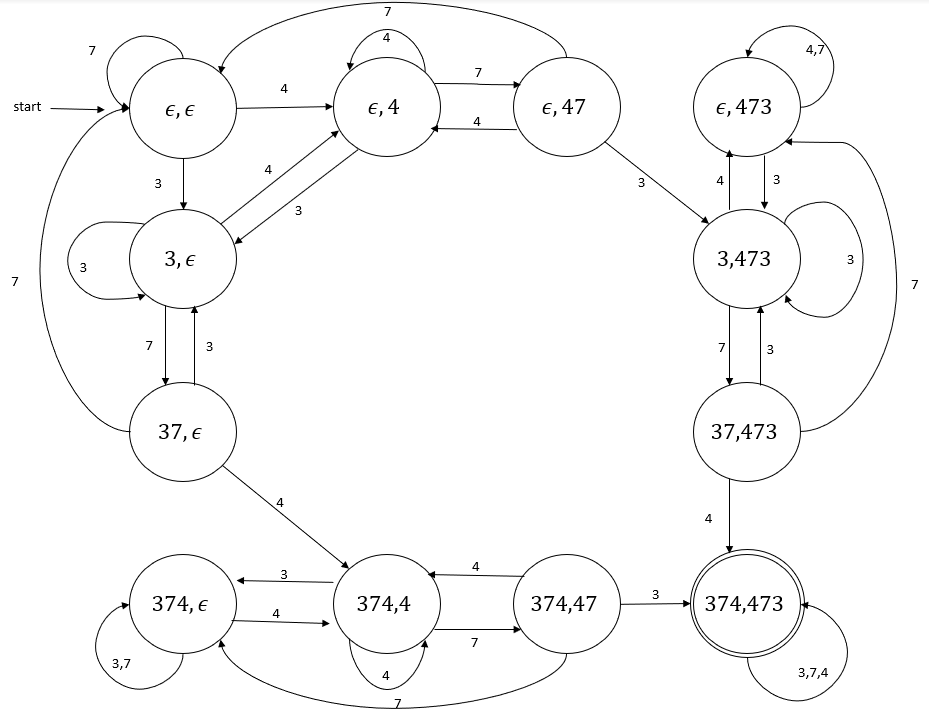
\includegraphics[width = 0.8\textwidth]{Q-7B}
\end{figure}

\question{7.C}

The follwing NFA accepts the language. The state is represents what the string ends with. All strings are accepted but if $4$ is read at state $37$, then there will be a $374$ substring and this won't be accpeted by the NFA.

\begin{figure}[hbt!]
	\centering
	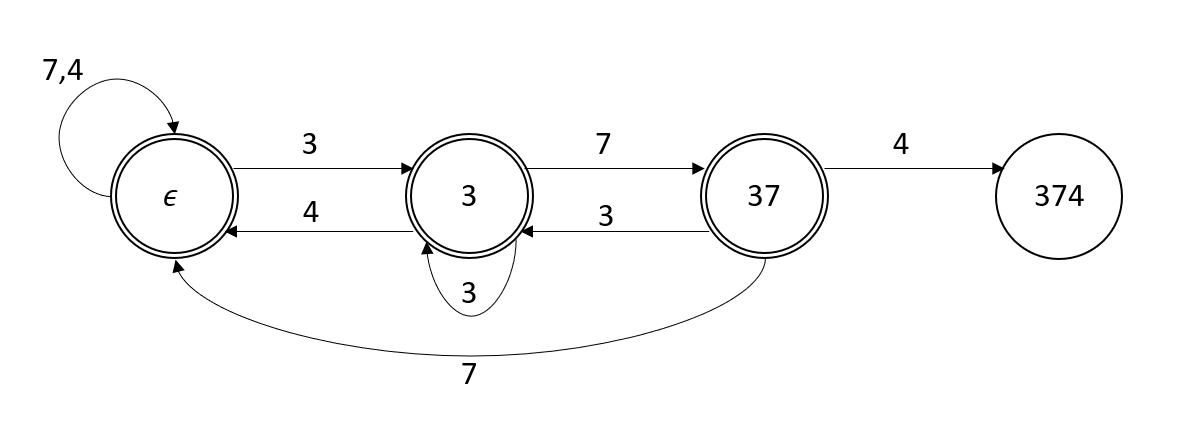
\includegraphics[width = 1\textwidth]{Q-7C}
\end{figure}

\question{7.D}

The folling NFA accepts the language. The state is represented with what the string ends with and the even or odd number of $7$s. On reading $7$, the state will transform from odd state to even state or even state to odd state while tracking the end string. On reading $3,4$, the end string state will be changed. Accpeting state is reached if and only if there's substring $374$ and number of $7$ is odd.

\begin{figure}[hbt!]
	\centering
	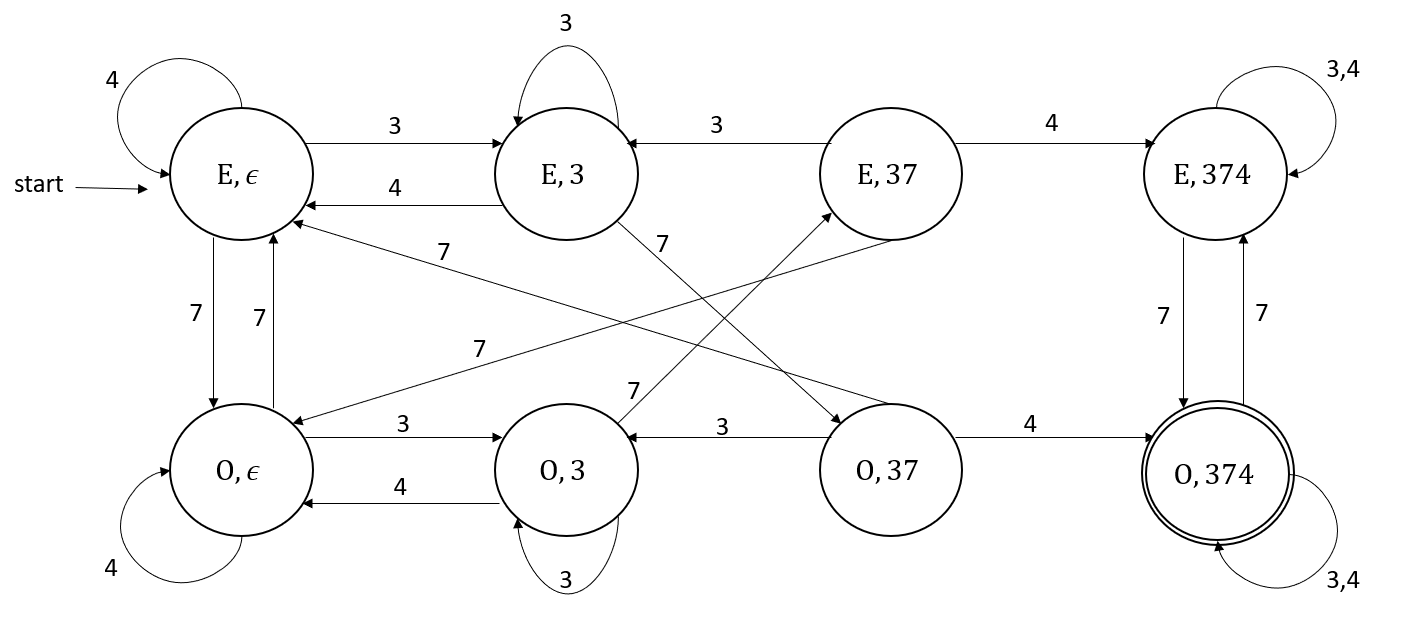
\includegraphics[width = 1\textwidth]{Q-7D}
\end{figure}

\question{7.E}

The folling NFA accepts the language. $q_0$ means maximal substring of consecutive $7$s is even and $q_1$ means maximal substring of consecutive $7$ is odd. When the substring of consecutive $7$s is odd and it reads $3$ or $4$. It will go to the rejecting state $\emptyset$. This makes sure that every maximal substring of consecutive $7$ is even in size.


\begin{figure}[hbt!]
	\centering
	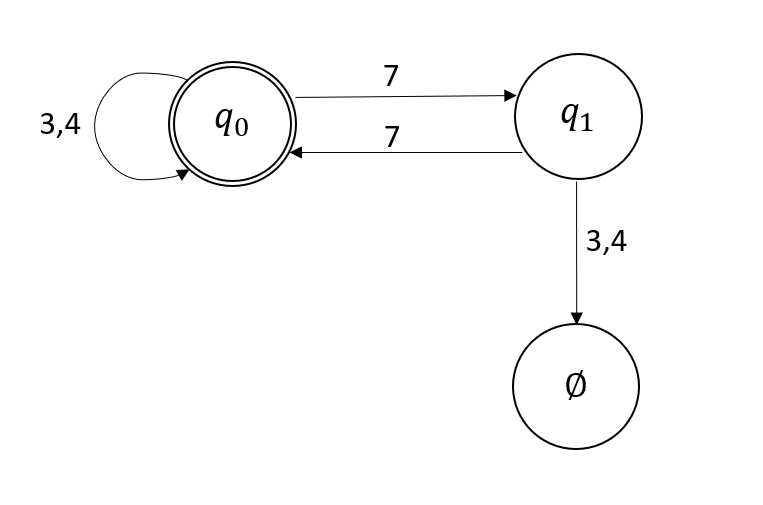
\includegraphics[width = 0.7\textwidth]{Q-7E}
\end{figure}

\question{8.A}\\
$\bullet$ \textbf{Intuition:} We can just exchange all the "1" in the L with "$\epsilon$".\\
$\bullet$ \textbf{Answer:}Set NFA $N_1=(\sum_1,Q_1,\delta_1,s_1,A_1)$

	Then NFA accepts DelOnes(L), so we can get:
	
	$\bullet$ $Q_1 = Q$

	$\bullet$ $\delta_1(q,0) = \delta(q,0)$, $\delta_1(q,\epsilon) = \delta(q,1)$, $\delta_1(q,1) = \emptyset $

	$\bullet$ $s_1 = s$

	$\bullet$ $A_1 = A$\\
	

\question{8.B}\\
$\bullet$ \textbf{Intuition:} We can just connect the state machine of "$x$" and the state machine of "$y$". We can add an "$\epsilon$" arrow between the "$x$ state machine's accepting state" and the "$y$ state machine's start state". 
That also means that we can use two DFA M. For one of them, we can swap all the transition function, and swap the start state and the accept state to get an DFA $M_2$. Then, we connect the accept state of $M$ with the new start state of $M_2$ by using $\epsilon$.\\
$\bullet$ \textbf{Answer:}Set $L_2=\{y \ \vline\ y \in L\}$ which is accepted by $M_2$. $M_2=(\sum,Q_2,\delta_2,s_2,A_2)$ Set $L_3=\{x \ \vline\ x \in L\}$ which is accepted by $M_3$. $M_3=(\sum,Q_3,\delta_3,s_3,A_3)$. 

	$\bullet$ $Q_2 = Q_3 = Q$

	$\bullet$  $\delta_2(q,a) = \delta_3(q,a) =\delta(q,a) $

	$\bullet$ $s_2 = s_3 = s$

	$\bullet$ $A_2 = A_3 = A$\\

	Set NFA $N_4=(\sum,Q_4,\delta_4,s_4,A_4)$,then NFA accepts ThereAndBack(L), so we can get:
	
	$\bullet$ $Q_4 = Q \times Q \times \{xs,ys\}$

	$\bullet$  $\delta_4((q,xs),a) = (\delta((q,xs),a),xs)$
 
	$\bullet$	$\delta_4(\delta((q,ys),a),a) = (q,ys)$

	$\bullet$	$\delta_4((a_3,xs)$,$\epsilon) = \{a_2 \ \vline\ a_2 \in A_2\}$, $a_3 \in A_3$

	$\bullet$ $s_4 = s_3$

	$\bullet$ $A_4 =\{s_2\}$\\

\question{8.C}\\
$\bullet$ \textbf{Intuition:} set the state to double state (q,r) so that we can consider x and y.\\
$\bullet$ \textbf{Answer:}Set $L_5=$XOR$(L)$, which is accepted by $M_5$.
Set $M_5=(\sum,Q_5,\delta_5,s_5,A_5)$\\

	$\bullet$ $Q_5 = Q \times Q$

	$\bullet$  $\delta_5((q,r),1) = \{(\delta(q,0),\delta(r,1)),(\delta(q,1),\delta(r,0))\}$, $\delta_5((q,r),0) = \{(\delta(q,1),\delta(r,1)),(\delta(q,0),\delta(r,0))\}$

	$\bullet$ $s_5 = (s, s)$

	$\bullet$ $A_5 = \{(q_1,q_2 \vline\ q_1 \in A$ and $q_2 \in A)\}$\\



\question{9.A}

\noindent
Let $F$ be the language $(01)^\ast$. \\
Let $x$ and $y$ be arbitrary strings in $F$. \\
Then $x=(01)^i$ and $y=(01)^j$ for some non-negative integers $i\neq j$. \\ 
Let $z=(10)^i (01)^i$. \\
Then $xz=(01)^i(10)^i(01)^i \in L$. \\ 
And $yz=(01)^j(10)^i(01)^i \notin L$, because $i \neq j$. \\ 
Thus, $F$ is a fooling set for $L$. \\
Because $F$ is infinite, $L$ cannot be regular. \\

\question{9.B}

\noindent
Let $F$ be the language $\{0^{2n}10^n\ \vline\ n \ge 0\}$. \\
Let $x$ and $y$ be arbitrary strings in $F$. \\
Then $x=0^{2i}10^i$ and $y=0^{2j}10^j$ for some non-negative integers $i\neq j$. Assume $j > i$. \\
Let $z=0^i$. \\
Then $xz=0^{2i}10^{2i} \in L$. \\ 
And $yz = 0^{2j}10^{i+j}\notin L$, because $k(i + j) \neq 2j$ for any integar $k$.  \\
Thus, $F$ is a fooling set for $L$. \\
Because $F$ is infinite, $L$ cannot be regular. \\

\question{9.C}

\noindent
Let $F$ be the language $\{a^{2^n}\ \vline\ n \ge 0\}$. \\
Let $x$ and $y$ be arbitrary strings in $F$. \\
As $j=\log_{2}{i}$, $i=2^j$. \\
Then $x=a^{2^i}$ and $y=a^{2^j}$ for some non-negative integers $i\neq j$. \\
Let $z=b^i$. \\
Then $xz=a^{2^{i}}b^i \in L$. \\
And $yz=a^{2^j}b^i\notin L$, because $\log_{2}{2^j} \neq i$. \\
Thus, $F$ is a fooling set for $L$. \\
Because $F$ is infinite, $L$ cannot be regular. \\

\question{9.D}

\noindent
Let $F$ be the language $\{0^{3n^2}\ \vline\ n \ge 0\}$. \\
Let $x$ and $y$ be arbitrary strings in $F$. \\
Then $x=0^{3i^2}$ and $y=0^{3j^2}$ for some non-negative integers $i\neq j$. \\
Let $z=0^{i^2}0^{2i}$. \\ 
Then $xz=0^{4i^2}0^{2i} \in L$. \\
And $yz=0^{3j^2+i^2}0^{2i} \notin L$, because $i \neq j \Rightarrow \sqrt{3j^2 + i^2} \neq 2i$. \\
Thus, $F$ is a fooling set for $L$. \\
Because $F$ is infinite, $L$ cannot be regular. \\

\question{9.E}

\noindent
Let $F$ be the language $a^*c$. \\
Let $x$ and $y$ be arbitrary strings in $F$. \\
Then $x=a^ic$ and $y=a^jc$ for some non-negative integers $i\neq j$. \\
Let $z=d^i$. \\
Then $xz=a^icd^i \in L$. \\
And $yz=a^i cd^j \notin L$, because $i = \#_a(w) \neq j$, where $w$ is $a^i$. \\
Thus, $F$ is a fooling set for $L$. \\
Because $F$ is infinite, $L$ cannot be regular. \\

\end{document}
